\documentclass{standalone}

\usepackage{tikz}
\usepackage{tkz-euclide}
\usetikzlibrary{calc}
\usetikzlibrary{positioning}
\usetikzlibrary{arrows.meta}

\usepackage{times}


\begin{document}
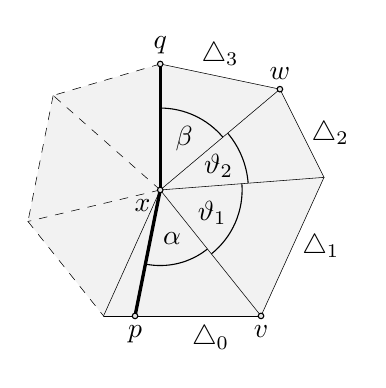
\begin{tikzpicture}[%
  >={Stealth[scale=1.0]},
  scale=0.8,
  % yscale=0.8,
]

  \tkzDefPoint(0.9, 2.0){A}
  \tkzDefPoint(0.0, 0.0){B}
  \tkzDefPoint(2.5, 0.0){C}
  \tkzDefPoint(3.5, 2.2){D}
  \tkzDefPoint(2.8, 3.6){E}
  \tkzDefPoint(0.9, 4.0){F}
  \tkzDefPoint(-0.8, 3.5){G}
  \tkzDefPoint(-1.2, 1.5){H}

  \tkzDefPointOnLine[pos=0.2](B,C)\tkzGetPoint{p}
  \tkzDefShiftPoint[A](0,0){x}
  \tkzDefShiftPoint[F](0,0){q}

  % \tkzDrawPolygon(A,B,C)
  % \tkzDrawPolygon(A,C,D)
  % \tkzDrawPolygon(A,D,E)
  % \tkzDrawPolygon(A,E,F)
  % \tkzDrawPolygon[dotted](A,F,G)
  % \tkzDrawPolygon[dotted](A,G,H)
  % \tkzDrawPolygon[dotted](A,H,B)

  \tkzFillPolygon[color=black!5](A,B,C)
  \tkzFillPolygon[color=black!5](A,C,D)
  \tkzFillPolygon[color=black!5](A,D,E)
  \tkzFillPolygon[color=black!5](A,E,F)
  \tkzFillPolygon[color=black!5](A,F,G)
  \tkzFillPolygon[color=black!5](A,G,H)
  \tkzFillPolygon[color=black!5](A,H,B)

  \tkzDrawSegments(B,C C,D D,E E,F)
  \tkzDrawSegments(A,B A,C A,D A,E A,F)
  \tkzDrawSegments[dashed](F,G G,H H,B)
  \tkzDrawSegments[dashed](A,G A,H)

  \tkzMarkAngle[size=1.2](p,x,C)
  \tkzLabelAngle[pos=0.8](p,x,C){$\alpha$}

  \tkzMarkAngle[size=1.3](C,x,D)
  \tkzLabelAngle[pos=0.9](C,x,D){$\vartheta_1$}
  \tkzMarkAngle[size=1.4](D,x,E)
  \tkzLabelAngle[pos=1.0](D,x,E){$\vartheta_2$}

  \tkzMarkAngle[size=1.3](E,x,q)
  \tkzLabelAngle[pos=0.9](E,x,q){$\beta$}

  \tkzDrawSegments[very thick](p,x x,q)
  \tkzDrawPoints(p,x,q,C,E)

  \tkzLabelPoint[below](p){$p$}
  \tkzLabelPoint[below left](x){$x$}
  \tkzLabelPoint[above](q){$q$}

  \tkzLabelPoint[below](C){$v$}
  \tkzLabelPoint[above](E){$w$}

  \tkzLabelSegment[below right](B,C){$\triangle_0$}
  \tkzLabelSegment[right](C,D){$\triangle_1$}
  \tkzLabelSegment[right](D,E){$\triangle_2$}
  \tkzLabelSegment[above](E,F){$\triangle_3$}

\end{tikzpicture}
\end{document}
